% Options for packages loaded elsewhere
\PassOptionsToPackage{unicode}{hyperref}
\PassOptionsToPackage{hyphens}{url}
\PassOptionsToPackage{dvipsnames,svgnames,x11names}{xcolor}
%
\documentclass[
  authoryear,
  preprint,
  3p]{elsarticle}

\usepackage{amsmath,amssymb}
\usepackage{iftex}
\ifPDFTeX
  \usepackage[T1]{fontenc}
  \usepackage[utf8]{inputenc}
  \usepackage{textcomp} % provide euro and other symbols
\else % if luatex or xetex
  \usepackage{unicode-math}
  \defaultfontfeatures{Scale=MatchLowercase}
  \defaultfontfeatures[\rmfamily]{Ligatures=TeX,Scale=1}
\fi
\usepackage{lmodern}
\ifPDFTeX\else  
    % xetex/luatex font selection
\fi
% Use upquote if available, for straight quotes in verbatim environments
\IfFileExists{upquote.sty}{\usepackage{upquote}}{}
\IfFileExists{microtype.sty}{% use microtype if available
  \usepackage[]{microtype}
  \UseMicrotypeSet[protrusion]{basicmath} % disable protrusion for tt fonts
}{}
\makeatletter
\@ifundefined{KOMAClassName}{% if non-KOMA class
  \IfFileExists{parskip.sty}{%
    \usepackage{parskip}
  }{% else
    \setlength{\parindent}{0pt}
    \setlength{\parskip}{6pt plus 2pt minus 1pt}}
}{% if KOMA class
  \KOMAoptions{parskip=half}}
\makeatother
\usepackage{xcolor}
\setlength{\emergencystretch}{3em} % prevent overfull lines
\setcounter{secnumdepth}{5}
% Make \paragraph and \subparagraph free-standing
\ifx\paragraph\undefined\else
  \let\oldparagraph\paragraph
  \renewcommand{\paragraph}[1]{\oldparagraph{#1}\mbox{}}
\fi
\ifx\subparagraph\undefined\else
  \let\oldsubparagraph\subparagraph
  \renewcommand{\subparagraph}[1]{\oldsubparagraph{#1}\mbox{}}
\fi


\providecommand{\tightlist}{%
  \setlength{\itemsep}{0pt}\setlength{\parskip}{0pt}}\usepackage{longtable,booktabs,array}
\usepackage{calc} % for calculating minipage widths
% Correct order of tables after \paragraph or \subparagraph
\usepackage{etoolbox}
\makeatletter
\patchcmd\longtable{\par}{\if@noskipsec\mbox{}\fi\par}{}{}
\makeatother
% Allow footnotes in longtable head/foot
\IfFileExists{footnotehyper.sty}{\usepackage{footnotehyper}}{\usepackage{footnote}}
\makesavenoteenv{longtable}
\usepackage{graphicx}
\makeatletter
\def\maxwidth{\ifdim\Gin@nat@width>\linewidth\linewidth\else\Gin@nat@width\fi}
\def\maxheight{\ifdim\Gin@nat@height>\textheight\textheight\else\Gin@nat@height\fi}
\makeatother
% Scale images if necessary, so that they will not overflow the page
% margins by default, and it is still possible to overwrite the defaults
% using explicit options in \includegraphics[width, height, ...]{}
\setkeys{Gin}{width=\maxwidth,height=\maxheight,keepaspectratio}
% Set default figure placement to htbp
\makeatletter
\def\fps@figure{htbp}
\makeatother

\usepackage{booktabs}
\usepackage{longtable}
\usepackage{array}
\usepackage{multirow}
\usepackage{wrapfig}
\usepackage{float}
\usepackage{colortbl}
\usepackage{pdflscape}
\usepackage{tabu}
\usepackage{threeparttable}
\usepackage{threeparttablex}
\usepackage[normalem]{ulem}
\usepackage{makecell}
\usepackage{xcolor}
\usepackage{todonotes,mathtools,bm,amsmath,mathpazo}
\mathtoolsset{showonlyrefs}
\setlength{\parindent}{0cm}
\makeatletter
\makeatother
\makeatletter
\makeatother
\makeatletter
\@ifpackageloaded{caption}{}{\usepackage{caption}}
\AtBeginDocument{%
\ifdefined\contentsname
  \renewcommand*\contentsname{Table of contents}
\else
  \newcommand\contentsname{Table of contents}
\fi
\ifdefined\listfigurename
  \renewcommand*\listfigurename{List of Figures}
\else
  \newcommand\listfigurename{List of Figures}
\fi
\ifdefined\listtablename
  \renewcommand*\listtablename{List of Tables}
\else
  \newcommand\listtablename{List of Tables}
\fi
\ifdefined\figurename
  \renewcommand*\figurename{Figure}
\else
  \newcommand\figurename{Figure}
\fi
\ifdefined\tablename
  \renewcommand*\tablename{Table}
\else
  \newcommand\tablename{Table}
\fi
}
\@ifpackageloaded{float}{}{\usepackage{float}}
\floatstyle{ruled}
\@ifundefined{c@chapter}{\newfloat{codelisting}{h}{lop}}{\newfloat{codelisting}{h}{lop}[chapter]}
\floatname{codelisting}{Listing}
\newcommand*\listoflistings{\listof{codelisting}{List of Listings}}
\makeatother
\makeatletter
\@ifpackageloaded{caption}{}{\usepackage{caption}}
\@ifpackageloaded{subcaption}{}{\usepackage{subcaption}}
\makeatother
\makeatletter
\@ifpackageloaded{tcolorbox}{}{\usepackage[skins,breakable]{tcolorbox}}
\makeatother
\makeatletter
\@ifundefined{shadecolor}{\definecolor{shadecolor}{rgb}{.97, .97, .97}}
\makeatother
\makeatletter
\makeatother
\makeatletter
\makeatother
\journal{Journal of Service Research}
\ifLuaTeX
  \usepackage{selnolig}  % disable illegal ligatures
\fi
\usepackage[]{natbib}
\bibliographystyle{elsarticle-harv}
\IfFileExists{bookmark.sty}{\usepackage{bookmark}}{\usepackage{hyperref}}
\IfFileExists{xurl.sty}{\usepackage{xurl}}{} % add URL line breaks if available
\urlstyle{same} % disable monospaced font for URLs
\hypersetup{
  pdftitle={Hierarchical Time Series Forecasting in Emergency Medical Services},
  pdfkeywords={healthcare, emergency services, forecast
reconciliation, ambulance demand, regression},
  colorlinks=true,
  linkcolor={blue},
  filecolor={Maroon},
  citecolor={Blue},
  urlcolor={Blue},
  pdfcreator={LaTeX via pandoc}}

\setlength{\parindent}{6pt}
\begin{document}

\begin{frontmatter}
\title{Hierarchical Time Series Forecasting in Emergency Medical
Services}


\cortext[cor1]{Corresponding author}
        
\begin{abstract}
Accurate forecasts of ambulance demand are crucial inputs when planning
and deploying staff and fleet. Such demand forecasts are required at
national, regional, and sub-regional levels, and must take account of
the nature of incidents and their priorities. These forecasts are often
generated independently by different teams within the organization. As a
result, forecasts at different levels may be inconsistent, resulting in
conflicting decisions and a lack of coherent coordination in the
service. To address this issue, we exploit the hierarchical and grouped
structure of the demand time series and apply forecast reconciliation
methods to generate both point and probabilistic forecasts that are
coherent and use all the available data at all levels of disaggregation.
The methods are applied to daily incident data from an ambulance service
in Great Britain, from October 2015 to July 2019, disaggregated by
nature of incident, priority, managing health board, and control area.
We use an ensemble of forecasting models and show that the resulting
forecasts are better than any individual forecasting model. We validate
the forecasting approach using time series cross validation.
\end{abstract}





\begin{keyword}
    healthcare \sep emergency services \sep forecast
reconciliation \sep ambulance demand \sep 
    regression
\end{keyword}
\end{frontmatter}
    \ifdefined\Shaded\renewenvironment{Shaded}{\begin{tcolorbox}[sharp corners, interior hidden, frame hidden, boxrule=0pt, borderline west={3pt}{0pt}{shadecolor}, enhanced, breakable]}{\end{tcolorbox}}\fi

\hypertarget{sec-intro}{%
\section{Introduction}\label{sec-intro}}

A failure to match available resources to demand in Emergency Medical
Services (EMS) results in patient flow problems, with serious
consequences for patients, staff, and the entire care system
\citep{ekstrom2015forecasting, ROSTAMITABAR20221197}. Demand forecasting
in EMS helps service planners to avoid the mismatch, potentially
providing massive savings in costs and lives, and leading to better
patient outcomes. Accurate daily demand forecasting enables planners and
decision-makers to manage resources to meet anticipated patients,
reconfigure units, and redeploy staff and vehicles as necessary.

Demand forecasts at EMS are typically required at multiple levels of an
organization to inform various planning and decision-making processes
\citep{hulshof2012taxonomic}. There are some planning processes at the
national level (strategic and long-term) such as workforce resource
planning and budgeting; sub-national, regional, or healthcare level
(tactical and medium-term) such as temporary capacity expansions,
resource sharing; and hospital or station level (operational and
short-term) such as planning rosters for staff and ambulance deployment.
Demand forecasts might also be required at different levels for a
specific area of interest such as the nature of demand or the priority
level. Moreover, the time series data in EMS has an inherent
hierarchical and grouped structure to support such forecasting
requirements. Demand for emergency medical services at the national
level can be disaggregated in a geographical hierarchy into
sub-national, regions, health boards, and stations/hospitals, or divided
into groups such as the nature of incidents or demand priority.
Forecasts produced at both higher and lower levels of hierarchies are
necessary for effective decision-making in EMS. For example, control
area EMS forecasts can inform strategic decisions about how to allocate
limited resources to lower levels, such as health boards and
stations/hospitals. At the lower levels, hospitals or ambulance stations
could use such forecasts to plan for staffing and resource allocation,
ambulance dispatching, staff-to-shift assignment, staff rescheduling
based on the anticipated volume and priority and nature of incidents.
Additionally, generating forecasts at lower levels could potentially
improve the accuracy of the high-level forecasts, by providing more
detailed information on the nature and priority of incidents. This could
help to identify patterns in demand that may not be apparent at the
higher level. Therefore, employing forecasting techniques that consider
the hierarchical and/or grouped patterns of time series in EMS aligns
naturally, offering the possibility to enhance forecast accuracy and
facilitate coordination.

To illustrate the problem, let's consider a very simple example where we
have an EMS provider with a national level of governance, and two
regions (A and B), each with a health board and a station. There is a
total national budget to be split between the regions in proportion to
the forecast number of incidents in each region. The two regions have
very different incident patterns, and so must be forecast using
different models. However, the data are noisy at regional level, so the
national forecasts are best obtained by summing the demand from the two
regions. The resulting national forecasts are not equal to the sum of
the regional forecasts, and so are not coherent. In fact, the national
forecasts show a decreasing trend in demand, and so the national
governing body decides to cut the budget for the next year. But neither
of the regional forecasts shows a trend, and so the regions argue that
the budget cut is unfair. In addition, Region A has much more variable
demand than Region B, and so to cope with periods of peak demand, Region
A needs to hold more resources in reserve. So the budget distribution
needs to be made in a way that ensures the probability of each region
being unable to meet demand is equal. Our solution to this problem is to
use a hierarchical forecasting approach that ensures the forecasts are
probabilistically coherent. Then any trends or other forecast
characteristics at national level will also be reflected in the regional
forecasts, and the probabilistic forecasts allow for the different
levels of uncertainty in the two regions. Budget can be allocated by
controlling the probability of demand exceeding available resources,
rather than being simply in proportion to the expected demand.

Despite a large number of studies dedicated to forecasting for EMS
\citep{mingliterature2022, gul2020exhaustive, ibrahim2016modeling, wargon2009systematic},
the hierarchical data structure has been largely ignored, and the main
focus has been on producing independent (base) forecasts at a single
level. Generating independent forecasts can result in a lack of
consistency and coordination, and therefore leads to less effective
planning and decision making.

With hierarchical forecasting, plans at any level are based on coherent
forecasts and therefore can be aligned. Implementing and sustaining
improvements in EMS require alignments and coordination between
different stakeholders, without which teams operate in isolation leading
to conflicts, duplication work, rework, or work that runs counter to the
overall goal to improve the quality of delivery service. Hierarchical
forecasting framework can be used as a tool to improve coordination
between teams across the care services at the national, sub-national,
regional and local levels. The hierarchical forecasting approaches not
only create consistent forecasts but are usually also more accurate than
the independent (base) forecasts \citep{hyndman2011optimal}. To our
knowledge, there has been no previous research involving hierarchical
and grouped forecasting in the entire field of forecasting for
healthcare management.

In this paper, we address this gap by investigating the application of
hierarchical forecasting approaches in the EMS using daily time series
of attended incidents from 2015 to 2019 in a major ambulance service in
Great Britain. The data has hierarchical and grouped structures, with
hierarchies at the national, control (i.e.~sub-national), and health
board (i.e.~regional) levels, as well as groups by priority and nature
of incidents. We produce consistent point forecasts and forecast
distributions for all levels over 84 days horizon, which is critical for
an effective planning and associated risk management. We compare the
point and probabilistic forecast accuracy of the independent forecasts,
bottom-up and optimal reconciliation approaches. We first generate
independent/base forecasts using Exponential Smoothing State Space
(ETS), Poisson regression using Generalized Linear Model (GLM) and
tscount (TSGLM), a simple empirical distribution and an ensemble method,
followed by applying bottom-up and optimal reconciliation approaches.
Forecast performance is assessed by the Mean Absolute Scaled Error
(MASE) and Mean Squared Scaled Error (MSSE) for point forecasts and
Continuous Ranked Probability Scores (CRPS) for the probabilistic
forecasts. This paper complies with reproducibility principles
\citep{stodden2013best, boylan2015reproducibility}. We provide the R
codes for the proposed models and benchmarks. Therefore, they can be
applied to any healthcare service (e.g., emergency department, primary
or social care) subject to the time series having a hierarchical and/or
grouped structure. While our research focuses on emergency medical
services, it is important to emphasize the suggested framework's
adaptability, which expands its relevance to a variety of service
sectors such as supply chains, tourism, finance, and call centers. Our
approach can be generalized in cases with hierarchically structured
and/or grouped time series data, which is common in many service
sectors.

The remainder of this article is structured as follows: In
Section~\ref{sec-lit}, we provide a brief review of the literature and
discuss its limitation to position our work; in
Section~\ref{sec-experiment}, we present the experiment design
describing the data set, forecasting methods and forecast evaluation
metrics. In Section~\ref{sec-htc}, we discuss the hierarchical time
series forecasting approaches to generate both point and probabilistic
forecasts. In Section~\ref{sec-results}, we present and discuss our
results; in Section~\ref{sec-conclusion}, we summarize our findings and
present ideas for future research.

\hypertarget{sec-lit}{%
\section{Research background}\label{sec-lit}}

Emergency medical services (EMS) are a critical component in the
delivery of urgent medical care to communities. An effective service
delivery requires accurate resource planning that generally relies on
demand forecasts at operational, tactical, and strategic levels. There
is a substantial number of studies on the application of time series
forecasting in the Emergency Medical Services. For example,
\citet{ibrahim2016modeling} provide an extensive review of the models
used in forecasting call volume arrivals. Another important area is
related to forecasting ambulance demand. Although the definition of
demand might not be always clearly stated, this is typically referring
to a situation where a physical resource has been deployed to respond to
an incident. This might be also called \emph{attended incidents}.
Another demand related variable is verified incidents; these are all
incidents that require an action: either by sending a physical vehicle,
responding via the Clinical Support Desk, requesting an external
provider to respond to it, or forwarding it to other channels such as
police, firefighters, or general practitioners. Our study is aligned
with this stream of literature. Another similar area that has received
considerable attention is Emergency Department forecasting; we refer
interested readers to \citet{mingliterature2022},
\citet{gul2020exhaustive}, and \citet{wargon2009systematic} for
extensive reviews of the relevant literature. In this section, we
provide a brief review of studies on forecasting ambulance demand in
EMS.

There are generally two main streams of research related to forecasting
ambulance demand in EMS: (i) the first stream focuses on the application
of time series methods and regression approaches to forecasting
aggregate ambulance demand \citep{vile2012predicting, sasaki2010using};
and (ii) the second stream considers forecasting EMS demand in finer
temporal and geographical granularities by employing temporal-spatial
prediction methods \citep{zhou2016predicting, zhou2016predictinglit}.
The focus of our study is related to the first stream of research.

\citet{sasaki2010using} develop a multivariable regression model to
estimate future EMS demands. In addition to the historical demand, the
population census for different age groups and counts of the number of
companies employing more than five people are included in the
regression. The census variables describe groups who are more likely to
need an ambulance. A stepwise ordinary least squares regression analysis
is used for estimating the parameter and generating forecasts. The only
performance measure reported in this study is \(R^2\), which is not an
effective measure of forecast accuracy \citep[p457]{armstrong01}. The
research design of this study is not rigorous and the study is not
reproducible. \citet{vile2012predicting} explore using a Singular
Spectrum Analysis (SSA) method to generate forecasts of the EMS demand
at the national level for 7-day, 14-day, 21-day, and 28-day forecast
horizons using data provided by an ambulance service in Great Britain.
The performance of this approach is compared to Auto-Regressive
Integrated Moving Average (ARIMA) and Holt-Winters time series methods
using Root Mean Squared Error (RMSE). They concluded that point
forecasts generated by SSA are more accurate for longer-term, but that
ARIMA and Holt-Winters performance is superior for shorter-term
horizons. \citet{vile2016time} further develop a decision support system
to integrate forecasts generated by SSA. However, the study does not
compare and contrast the performance of forecasting methods based on
utility measures such as cost, resource utilization and response time.
The tool contains options that allow generating forecasts at various
levels of granularity; however, it ignores the structure of the
hierarchical and grouped relationships, preventing aligned decision
making and coordination. \citet{al2021empirical} utilises data from the
Welsh Ambulance Service to explore the forecast accuracy of four
forecasting approaches: ARIMA, Holt Winters, Multiple Regression, and
Singular Spectrum Analysis (SSA) in predicting call volume demand. The
aim is to compare these approaches with the current method across
various planning horizons (7 days, 30 days, and 90 days) for both total
call volume and category-specific demand. Forecast accuracy performance
is evaluated using root mean square error (RMSE) and mean absolute
percentage error (MAPE). The findings indicate that ARIMA performs the
best in predicting weekly and monthly demand. However, when it comes to
long-term demand, the SSA method proves to be the most effective.
\citet{ibrahim2016modeling} conducted a case study to assess the
effectiveness of multiple forecasting methods: the multiplicative
univariate forecasting model (MU), univariate mixed-effects model (ME),
and two variations of bivariate mixed-effects models (BME). Call centre
data were utilized to forecast for periods of 1, 7, and 14 days ahead,
using only a limited dataset of 42 days. The performance of these
forecasting methods was evaluated using two metrics: RMSE for point
forecasts and coverage probability for the 95\% prediction interval. The
findings indicate that the ME consistently produces the most accurate
point forecasts. On the other hand, BME models demonstrate superior
coverage probabilities when forecasting for one day or one week ahead.
For a two-week leading period, MU shows better coverage probability.

\citet{9659837} investigate forecasting EMS demand in a high
Spatio-temporal resolution of 1km\(^2\) spatial regions and 1-hr time
intervals using total incidents in Oslo, Norway, from 1 January 2015 to
11 February 2019. They used multi-layer perceptron (MLP) and long
short-term memory (LSTM) models to forecast the EMS demand, and compare
the results to simple aggregation methods and baselines. The point
forecast accuracy is evaluated using Mean Absolute Error (MAE) and Mean
Squared Error (MSE), and the forecast distribution is measured by
Categorical Cross-Entropy. They found that Neural Network models
performed better in producing point forecasts, while a distribution
baseline method based on the spatial distribution of the incidents
across all time steps provided more accurate forecast distributions.
\citet{zhou2016predictinglit} proposed three methods based on Gaussian
mixture models, kernel density estimation, and kernel warping to predict
hourly data 4 weeks ahead for a 1km\(^2\) spatial region. Two years of
incidents from Toronto, Canada (years 2007 and 2008 with 391,296 events)
and Melbourne, Australia were used to build the model and examine the
performance on test data using mean negative log-likelihood. They show
that forecasts generated by the proposed methods were significantly more
accurate than the current industry practice (a simple averaging
formula). \citet{grekousis2019will} investigated the combination of
spatial analysis methods with data mining techniques based on an
improved Hungarian algorithm and a MLP neural network to identify the
most likely locations of future emergency events. The proposed approach
was tested using data from 2851 events attended by the EMS in Athens,
Greece, over 24 weeks. They showed that 23\% of real emergency events
lie within 50 meters of the predicted ones and nearly 70\% of the real
emergency events lie no further than 150 meters away, which is rather
accurate given the granularity of the problem at the city level.

Table~\ref{tbl-literature} provides a summary of some studies in the
literature on forecasting in Emergency Medical Services. We note a
number of limitations in the literature of EMS forecasting, that
encourage us to undertake this research. These limitations are
summarized as following:

\begin{enumerate}
\def\labelenumi{\arabic{enumi}.}
\item
  Current studies ignore the inherent hierarchical and/or grouped
  structure of the time series data, and the relationship between series
  at different levels of hierarchy. While the hierarchical forecasting
  methodology has been developed and applied in various domains over the
  past 10 years \citep{panagiotelis2023probabilistic}, it has never been
  explored in this area.
\item
  Current research is mainly concerned with generating point forecasts
  at a single level of hierarchy. There is a lack of studies considering
  the entire forecast distribution of daily ambulance demand for the
  whole hierarchy to better represent the uncertainty of future demand,
  providing a risk management tool for planners.
\item
  Reproducibility is still a major challenge in EMS forecasting, as it
  is unlikely that any reader can reproduce prior studies without the
  help of the authors of those papers.
\item
  Another limitation is related to the generated forecasts not being on
  the sample space of non-negative counts. Since actual ambulance counts
  cannot be negative or non-integer, ambulance demand forecast
  distributions should reflect the data. Of course, point forecasts
  represent means, so they should be non-negative, but may be
  non-integer. While this might not be an issue when producing forecasts
  at a single level, producing non-negative count forecasts in a
  hierarchical/grouped structure is challenging and requires further
  investigation in the future.
\end{enumerate}

This paper concerns the problem of hierarchical forecasting in EMS and
generates and evaluates both point and probabilistic forecast across
different levels of the hierarchy, hence addressing some important gaps
identified in the literature.

\hypertarget{tbl-literature}{}
\begin{landscape}\begin{table}
\caption{\label{tbl-literature}Summary of some studies on forecasting in Emergency Medical Services }\tabularnewline

\centering\begingroup\fontsize{11}{13}\selectfont

\resizebox{\linewidth}{!}{
\begin{tabular}{lr>{\raggedright\arraybackslash}p{6em}>{\raggedright\arraybackslash}p{4em}>{\raggedright\arraybackslash}p{10em}>{\raggedright\arraybackslash}p{8em}lll}
\toprule
Reference & Year & Variable & Horizon & Method & Metric & Probabilistic & Reconciliation & Reproducibility\\
\midrule
Current study & 2023 & Ambulance demand & 84 days & Stationary,  Exponential Smoothing State Space (ETS), Poisson regression using Generalized Linear Model (GLM) and tscount (TSGLM), a simple empirical distribution and an ensemble method & MASE, MSSE, CRPS & YES & YES & YES\\
Al-Azzani et al. & 2021 & Call volume & 7 , 30 ,  90 days & ARIMA, Holt Winters, Multiple Regression, and Singular Spectrum Analysis & RMSE, MAPE & NO & NO & NO\\
Haugsbø et al. & 2021 & Ambulance demand in Spatio-temporal & 1hour & MLP, LSTM & MAE, MSE, Cross-Entropy & YES & NO & NO\\
Grekousis et al. & 2019 & Locations of incidents & 1 hour & MLP and Hungarian algorithm & RMSE & NO & NO & NO\\
Ibrahim et al. & 2016 & Call volume & 1, 7 , 14 days & multiplicative univariate forecasting, univariate mixed-effects, bivariate mixed-effects model, and bivariate mixed-effects & RMSE, prediction interval coverage & Partial & NO & NO\\
Vile et al. & 2012 & Ambulance demand & 7, 14, 21,  28 day & Singular Spectrum Analysis, ARIMA,  Holt-Winters & RMSE & NO & NO & NO\\
Sasaki et al. & 2010 & Ambulance demand & 5 years & OLS regression & R\textasciicircum{}2 & NO & NO & NO\\
\bottomrule
\end{tabular}}
\endgroup{}
\end{table}
\end{landscape}

\hypertarget{sec-experiment}{%
\section{Experiment setup}\label{sec-experiment}}

Planners in the ambulance service work with a planning horizon of 6
weeks. That is, planning is generally frozen for the next 42 days, so
any forecasts will only affect plans for the time period beyond the next
42 days. Consequently, the forecast horizon in this study is
\(2 \times 42 = 84\) days ahead, with performance evaluation assessed
based on the last 42 days and not the whole forecast period. The
forecasts are produced for various training and test sets using time
series cross-validation \citep{hyndman2021forecasting}.

In the following section, we discuss the dataset, describe the
forecasting methods used to generate base forecasts, and present the
point and probabilistic accuracy measures.

\hypertarget{sec-data}{%
\subsection{Data}\label{sec-data}}

The dataset used in this study is from a major ambulance service in
Great Britain. It contains information relating to the daily number of
attended incidents from 1 October 2015 to 31 July 2019, disaggregated by
nature of incidents, priority, the health board managing the service and
the control area (or region). Figure~\ref{fig-hierarchy} depicts both
the hierarchical and grouped structure of the data.
Figure~\ref{fig-hierarchy-1} illustrates the nested hierarchical
structure based on control area and health board and
Figure~\ref{fig-hierarchy-2} shows the grouped structure by priority and
the nature of incident.

\begin{figure}

\begin{minipage}[t]{0.56\linewidth}

{\centering 

\raisebox{-\height}{

\includegraphics{main_files/figure-pdf/fig-hierarchy-1.pdf}

}

}

\subcaption{\label{fig-hierarchy-1}Hierarchical structure: Attended
incidents in the whole country are disaggregated into 3 control areas
and then into 7 different healthboards, anonymized using two letters
(e.g.~AB)}
\end{minipage}%
%
\begin{minipage}[t]{0.02\linewidth}

{\centering 

~

}

\end{minipage}%
%
\begin{minipage}[t]{0.42\linewidth}

{\centering 

\raisebox{-\height}{

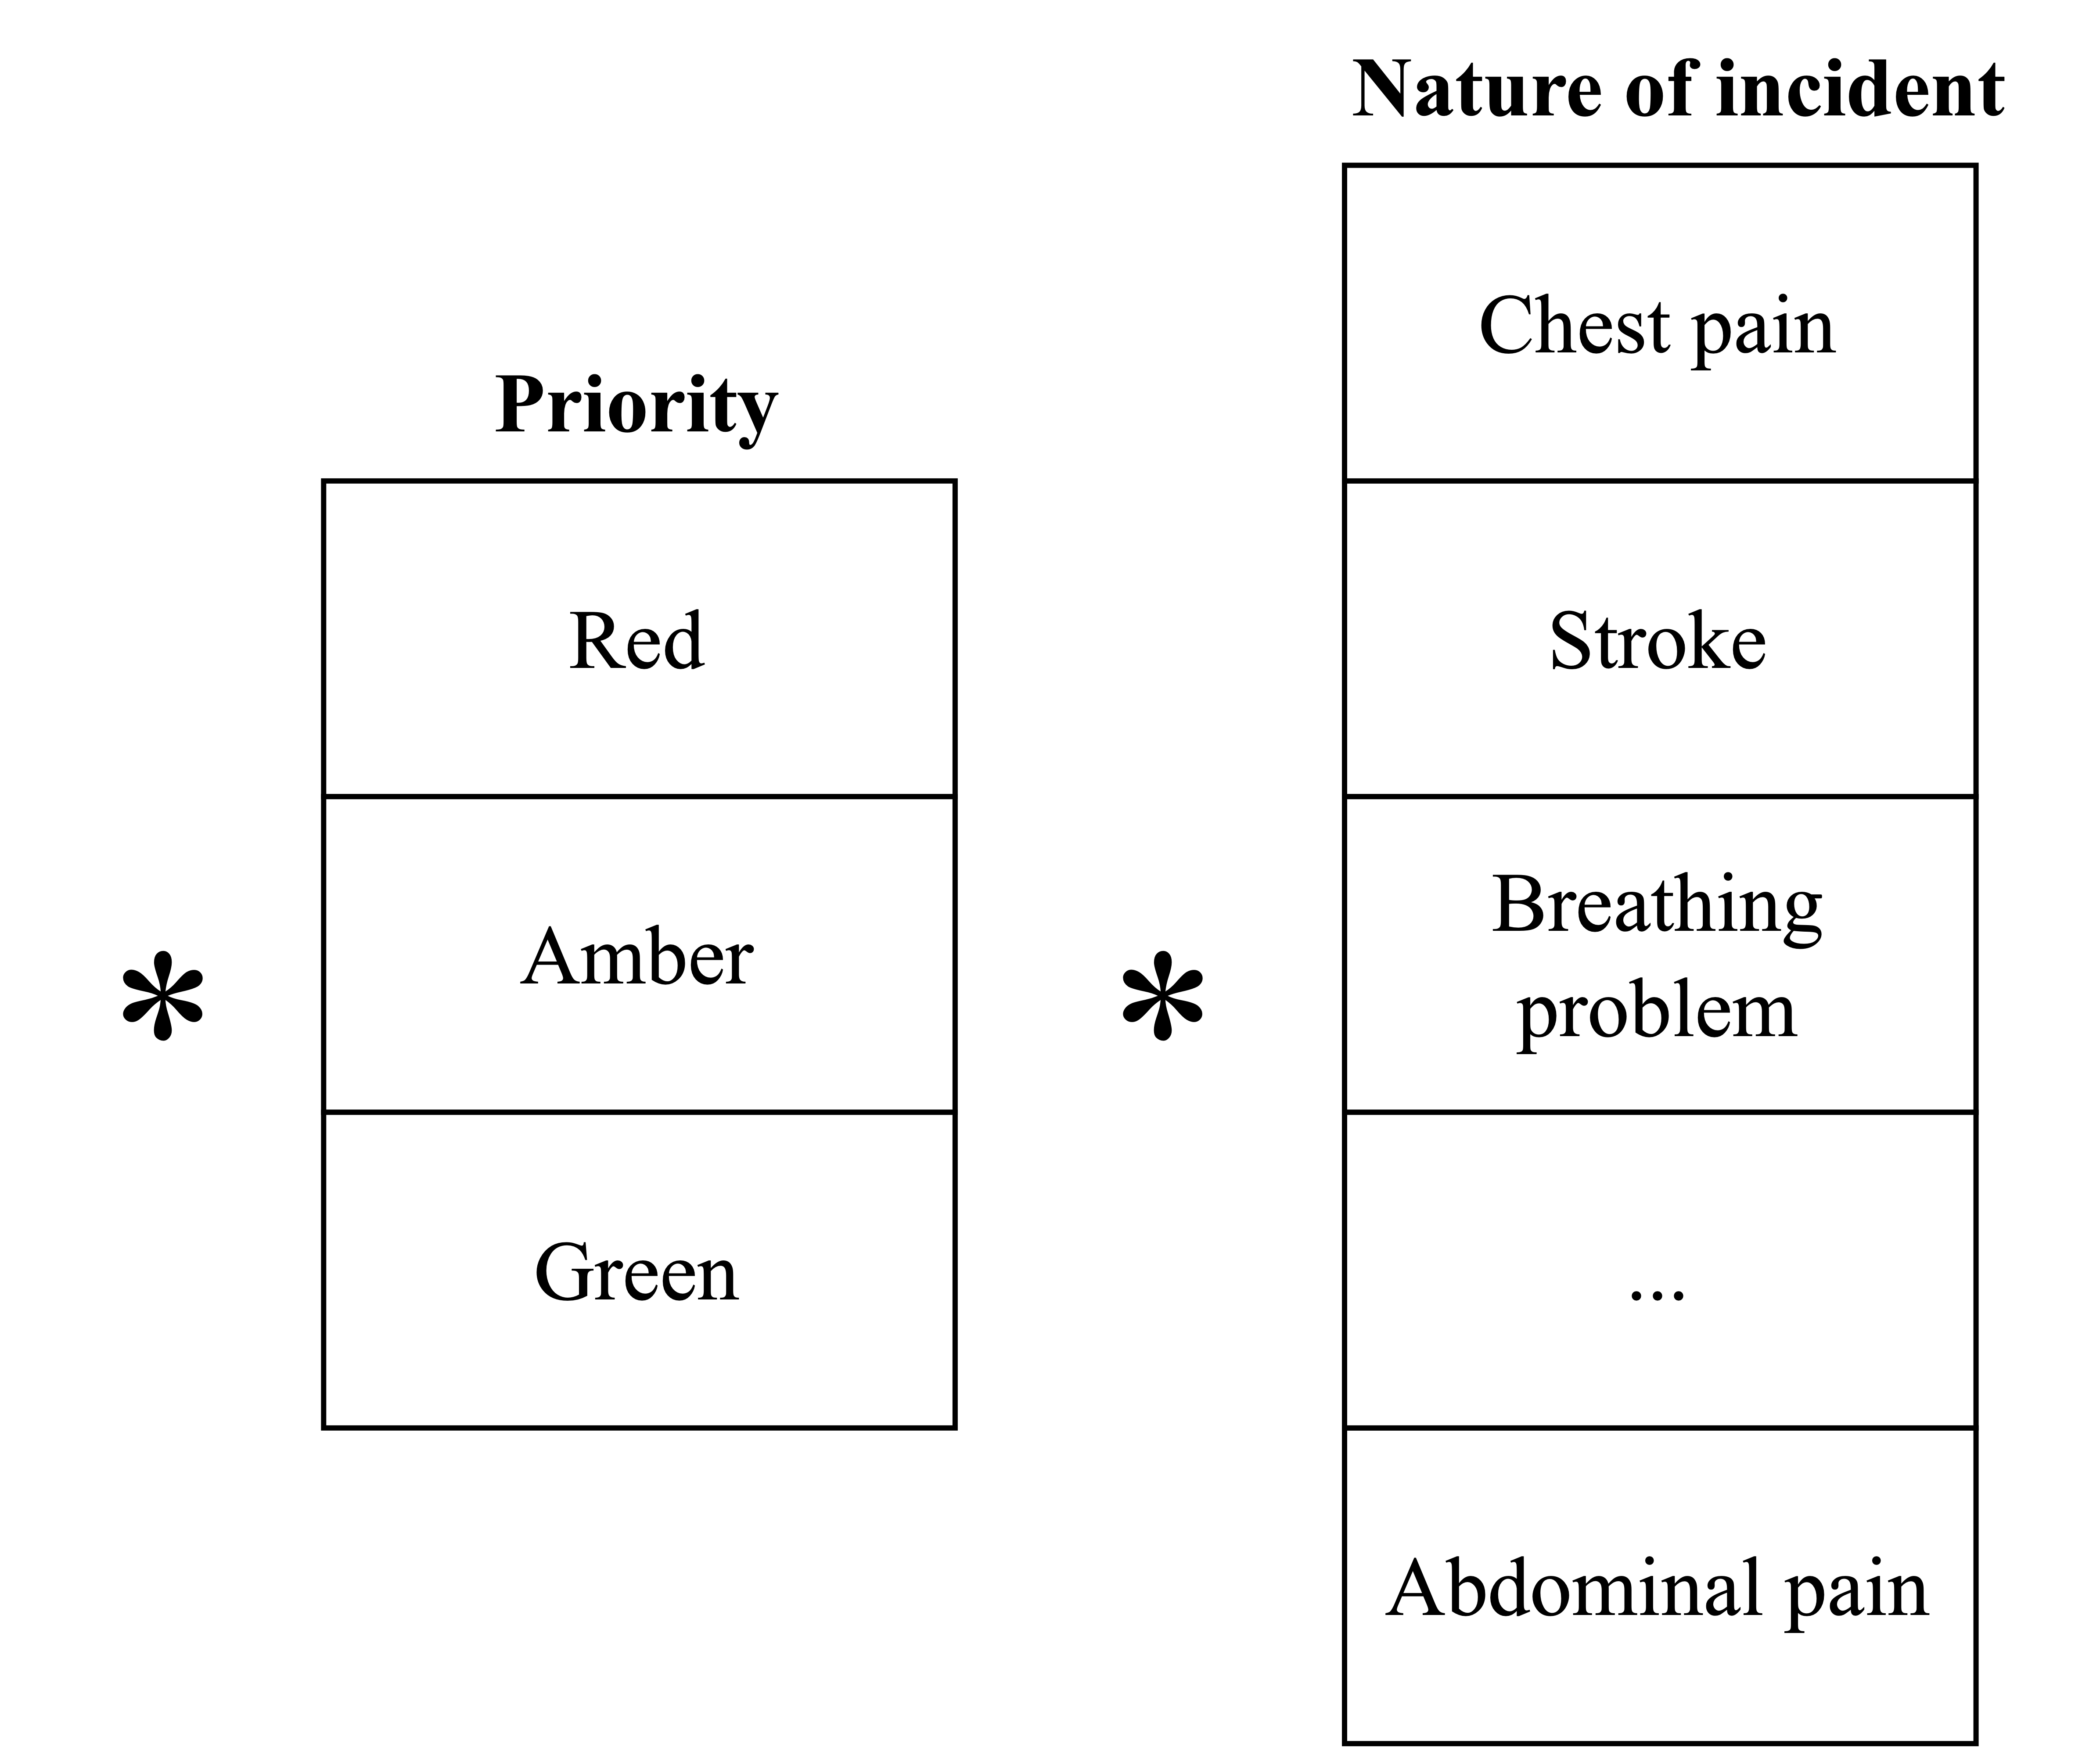
\includegraphics{../img/group.png}

}

}

\subcaption{\label{fig-hierarchy-2}Grouped structure: Incidents could be
grouped into priority (i.e.~Red, Amber \& Green) and the nature of
attended incident (i.e.~there are 35 different nature of incidents
including chest pain, breathing problems, heart attack, stroke, and so
on). The symbol * refers to the crossed attributes between hierarchical
and grouped levels.}
\end{minipage}%

\caption{\label{fig-hierarchy}The hierarchical and grouped structure of
attended incidents (ambulance demand).}

\end{figure}

Table~\ref{tbl-hierarchy} also displays the structure of data with the
total number of series at each level. At the top level, we have the
total attended incidents for the country. We can split these total
attended incidents by control area, by health board, by priority or by
nature of incident. There are 3 control areas breakdown by 7 local
health boards. Attended incident data are categorized into 3 priority
classes of red, amber, and green. There are also 35 different nature of
incidents such as chest pain, stroke, breathing problem, etc. In total,
across all levels of disaggregation, there are 1530 time series.

\hypertarget{tbl-hierarchy}{}
\begin{table}
\caption{\label{tbl-hierarchy}Number of time series in each level for the hierarchical \& grouped
structure of attended incidents }\tabularnewline

\centering
\begin{threeparttable}
\begin{tabular}{lr}
\toprule
Level & Number of series\\
\midrule
All country & 1\\
Control & 3\\
Health board & 7\\
Priority & 3\\
Priority * Control & 9\\
\addlinespace
Priority * Health board & 21\\
Nature of incident & 35\\
Nature of incident * Control & 105\\
Nature of incident * Health board & 245\\
Priority * Nature of incident & 104\\
\addlinespace
Control * Priority * Nature of incident & 306\\
Control * Health board * Priority * Nature of incident (Bottom level) & 691\\
Total & 1530\\
\bottomrule
\end{tabular}
\begin{tablenotes}
\item \textit{Note: } 
\item Due to certain combinations of the nature of incident with other variables, there is a lack of representation in the dataset. As a result, for example, instead of the calculation 3 * 35 = 105, it would be modified to 3 * 35-1 = 104.
\end{tablenotes}
\end{threeparttable}
\end{table}

Given the total number of time series, direct visual analysis is
infeasible. Therefore, we first compute features of all 1530 time series
\citep{m3pca} and display the strength of trend and weekly seasonality
strength in Figure~\ref{fig-feature}. Each point represents one time
series with the strength of trend in x-axis and the strength of
seasonality in y-axis. Both measures are on a scale of {[}0,1{]}.

In this paper, the strength of trend and seasonality were calculated
using the ``STL'' (Seasonal and Trend decomposition using Loess)
decomposition method, as described by \citet{mstl}. STL is a widely used
and flexible method for decomposing time series data into trend,
seasonal, and remainder components. The decomposition of a time series
\(y_t\) is written as \(y_t = T_t + S_{t} + R_t\), where \(T_t\) is the
smoothed trend component, \(S_t\) is the seasonal component and \(R_t\)
is a remainder component. The strength of trend is defined as:
\[F_T = \max\left(0, 1 - \frac{\text{Var}(R_t)}{\text{Var}(T_t+R_t)}\right)\]
For strongly trended data, the seasonally adjusted data should have much
more variation than the remainder component. Therefore
Var(\(R_t\))/Var(\(T_t+R_t\)) should be relatively small. But for data
with little or no trend, the two variances should be approximately the
same.

The strength of seasonality is defined similarly:
\[F_S = \max\left(0, 1 - \frac{\text{Var}(R_t)}{\text{Var}(S_{t}+R_t)}\right).\]
series with seasonal strength \(F_S\), close to 0 exhibits almost no
seasonality, while a series with strong seasonality will have \(F_S\)
close to 1 because Var(\(R_t\)) will be much smaller than
Var(\(S_t+R_t\)).

It is clear that there are some series showing strong trends and/or
seasonality, corresponding to series at the higher levels of the
hierarchy. The majority of series show low trend and seasonality. These
are time series belonging to the bottom series, series related to the
nature of incidents for a given control, health board and priority
level. Bottom series are dominated by noise with little or no systematic
patterns.

\begin{figure}

{\centering \includegraphics[width=0.7\textwidth,height=\textheight]{main_files/figure-pdf/fig-feature-1.pdf}

}

\caption{\label{fig-feature}The strength of the trend and weekly
seasonality in the time series of attended incidents. The scatter plot
shows a total of 1530 data points, with each point corresponding to a
specific time series.}

\end{figure}

In addition to displaying the trend and seasonality strength
\citep{hyndman2021forecasting}, we also visualize a few time series at
various levels of aggregation. Figure~\ref{fig-dataviz2} reveals
different information such as trend, seasonality, and noise. For
example, some series depict seasonality and trend, whereas some other
series report low volume of attended incidents and entropy, making them
more volatile and difficult to forecast. At the level on nature of
incidents combined with categories of other levels, there are many
series that contain zeros with low counts. As such, the data set
represents a diverse set of daily time series patterns.

\begin{figure}

{\centering \includegraphics[width=1\textwidth,height=\textheight]{main_files/figure-pdf/fig-dataviz2-1.pdf}

}

\caption{\label{fig-dataviz2}Daily time plot of attended incidents at
various levels. X-axis shows the date of incidents, consisting of 1400
data points (days) and y-axis shows the number of attended incidents.
The panels show data from the whole country (top panel), by control
area, by health board, by priority level, and by nature of incident.
Only four of the 35 nature of incident categories are shown to avoid too
much overplotting. Each time plot .}

\end{figure}

We consider several forecasting models that account for the diverse
patterns of the time series across the entire hierarchy. In developing
the forecasting models, the time series of holidays are also used in
addition to the attended incidents. We use public holidays, school
holidays and Christmas Day and New Year's Day as predictors of incident
attended. These types of holidays will affect peoples' activities and
may increase or decrease the number of attended incidents.

\hypertarget{forecasting-methods}{%
\subsection{Forecasting methods}\label{forecasting-methods}}

Given the presence of various patterns in the past attended incidents,
we consider three different forecasting models to generate the base
forecasts. Once the base forecasts are produced, hierarchical and
grouped time series methods are used to reconcile them across all
levels. We briefly discuss forecasting models in the following sections,
and the hierarchical forecasting methods are discussed in
Section~\ref{sec-htc}.

\textbf{Stationary:} We start with a simple forecasting approach,
assuming that the future days will be similar to past days. We use the
empirical distribution of the past daily attended incidents to create
the forecast distribution of future attended incidents. We have chosen
this ``stationary'' method as a benchmark due to its widespread usage
and simplicity, making it easily understandable for users. Forecasts
serve as inputs for various decision-making systems that frequently
employ simulations, wherein it is common to utilize the empirical
distribution of demand as a forecast. Additionally, the stationary
method has shown surprisingly high accuracy. Hence, any forecasting
approach that can offer superior results compared to the stationary
method would validate its practical use, otherwise there is no necessity
for employing more complex methods.

\textbf{Exponential Smoothing State Space model (ETS):} ETS models
\citep{hyndman2021forecasting} can combine trend, seasonality, and error
components in a time series through various forms that can be additive,
multiplicative or mixed. The trend component can be none (``N''),
Additive (``A'') or damped (``Ad''); the seasonality can be none
(``N''), Additive (``A''), or multiplicative (``M''); and the error term
can be additive (``A'') or multiplicative (``M''). To forecast the
attended incidents at each level, we use the \texttt{ets()} function in
the \texttt{forecast} package \citep{Rforecast, HK08} in R. To identify
the best model for a given time series, the \texttt{ets} function uses
the corrected Akaike's Information Criterion (AICc).

In our study, we use an automated algorithm to determine the suitable
configuration for the trend, seasonality, and error terms in each time
series. Specifically, we utilize the \texttt{ets()} function in the
forecast package of R, which employs Akaike's Information Criterion
(AIC) to identify the optimal model for each time series. Given the
large number of time series we work with (1530), it is impractical to
manually select the appropriate form for each component in every time
series. Consequently, the automated algorithm selects the best model
based on the unique characteristics of each individual time series. As a
result, a combination of additive or multiplicative forms for the
components are employed, depending on the specific attributes of each
time series.

Despite the popularity and the relevance of automatic \texttt{ETS} in
this study, it may produce forecast distributions that are non-integer
and include negative values, although the number of attended incidents
is always integer and non-negative. When using \texttt{ETS}, a time
series transformation approach could be used to generate strictly
positive forecasts, although forecast distributions will still be
non-integer. An alternative is to use forecasting models that produce
integer, non-negative forecasts. In the following section we present
Generalized Linear Models (GLMs) and Poisson time series regression to
produce count base forecasts.

\textbf{Generalized Linear Model (GLM):} GLMs are a family of models
developed to extend the concept of linear regression models to
non-Gaussian distributions \citep{Faraway2016}. They model the response
variable as a particular member of the exponential family, with the mean
being a transformation of a linear function of the predictors. One of
the models that is frequently used in practice to generate count
forecasts is Poisson regression.

Suppose the time series is denoted by \(y_1,\dots,y_T\), then the
Poisson GLM can be written as \begin{align*}
  y_t &\sim \text{Poisson}(\lambda_t) \\
  \text{where}\qquad
  \log(\lambda_t) &= \bm{x}_t'\bm{\beta},
\end{align*} and \(\bm{x}_t\) is a vector of covariates, \(\beta\) is a
vector of coefficients, and \(\lambda_t\) is the mean of the Poisson
distribution. In our model, these include cubic splines for the time
trend, day-of-week dummy variables (from Monday to Sunday), Fourier
terms to capture the yearly seasonality, dummy variables indicating
public holidays (1 when is a public holiday, 0 otherwise), school
holidays (1 when is a school holiday, 0 otherwise), and Christmas Day (1
when is Christmas Day, 0 otherwise) and New Year's Day (1 when is New
Year's Day, 0 otherwise). The Fourier terms are as defined in
\citet[Section 7.4]{hyndman2021forecasting}. This model takes account of
weekly seasonality and annual seasonality. Monthly seasonality in time
series data is extremely rare, and it does not exist in the ambulance
demand used in this study. There is no reason for occurrences to occur
more frequently at certain times of the month than others.

We fit a Poisson regression model using the function \texttt{glm()} from
the \emph{stats} package in R, with the argument
\texttt{family\ =\ poisson} to specify that we wish to fit a Poisson
regression model with a log link function.

\textbf{Poisson Regression using tscount (TSGLM):} We also consider
another Poisson regression model that takes into account serial
dependence. This model captures the short-range serial dependence by
including autoregressive terms in addition to the same covariates that
were used in the GLM model. To distinguish this from the previous GLM
model, we will refer to this model as \texttt{TSGLM}.

The Poisson TSGLM is similar to the GLM, with an additional
autoregressive component accounting for serial dependence. The term
serial dependence refers to instances in which the number of incidents
on a current day correlates with the number of incidents on previous
days. \begin{align*}
  y_t &\sim \text{Poisson}(\lambda_t) \\
  \text{where}\qquad
  \log(\lambda_t) &= (\bm{y}_{t-k}' , \bm{x}_t')\bm{\beta},
\end{align*} and \({y}_{t-k}\) is a vector of \(k\) lagged values. The
TSGLM model explicitly accounts for serial dependence by including
lagged values (i.e., past values) of the ambulance demand in the model.
This is important in EMS forecasting because it allows the model to
capture patterns in the data that are dependent on the past values of
the time series, which might not be captured via the predictor
variables.

We use the \texttt{tsglm()} function in the \texttt{tscount} package in
R \citep{JSSv082i05} to model the attended incidents. Again, the
logarithmic link function is used to ensure that the mean of the Poisson
distribution is always positive.

Provided accidents occur independently, they will inherently follow a
Poisson distribution \citep[p156--158]{feller1991introduction}. Hence,
it is reasonable to assume a Poisson distribution in this context. To
account for changes over time, we incorporate trend and seasonality
covariates, as well as public holiday effects, allowing the mean of the
Poisson distribution to vary. However, it is important to note that if
there are additional factors influencing the mean of the Poisson
distribution that are not accounted for in our model, we might observe
over- or under-dispersion in the data.

\textbf{Ensemble method:} Finally, one effective strategy for improving
forecast accuracy includes the simultaneous application of multiple
forecasting methods on a given time series, followed by combining the
forecasts rather than relying on separate forecasts generated by each
individual method \citep{clemen1989combining}. In this paper, we use an
ensemble method that combines the forecasts generated from the
Stationary, ETS, GLM, and TSGLM models using a simple average to form a
mixture distribution \citep{combinations}.

To generate forecast probability distributions using the above methods,
we use a form of bootstrapping, described in
\citet{panagiotelis2023probabilistic}. This involves simulating 1000
future sample paths from each of the models by bootstrapping the model
residuals, taking into account the cross-sectional correlations between
the different aggregated and disaggregated series. In this way, we can
generate an empirical distribution of forecasts for each model. The
ensemble forecast distribution is a simple mixture of these empirical
distributions.

It is important to emphasize that the aim of this study is not to
provide an exhaustive compilation of forecasting models or to promote a
particular model class. Instead, we have developed a flexible framework
that can accommodate any forecasting model. Our primary objective is to
demonstrate its practicality and effectiveness in integrating base
forecasts from any model and generating coherent forecasts within a
hierarchical structure.

\hypertarget{performance-evaluation}{%
\subsection{Performance evaluation}\label{performance-evaluation}}

To evaluate the performance of the various forecasting approaches, we
split the data into a series of ten training and test sets. We use a
time series cross-validation approach \citep{hyndman2021forecasting},
with a forecast horizon of 84 days, and each training set expanding in
42-day steps. The first training set uses all data up to 2018-04-25, and
the first test set uses the 84 days beginning 2018-04-26. The second
training set uses all data up to 2018-06-06, with the second test set
using the following 84 days. The largest training set ends on
2019-05-09, with the test set ending on 2019-07-31. Model development
and hyper-parameter tuning is performed using the training data and the
errors are assess using the corresponding test set. While we compute
forecast errors for the entire 12 weeks, we are most interested in the
last 42 days of each test set, because that corresponds to how forecasts
are generated for planning in practice. Forecasting performance is
evaluated using both point and probabilistic error measures.

The error metrics provided below consider a forecasting horizon denoted
by \(j\), representing the number of time periods ahead we are
predicting. In our study, this forecasting horizon ranges from 1 to 84
days, \(j= 1,2,\dots, 84\).

Point forecast accuracy is measured via the Mean Squared Scaled Error
(MSSE) and the Mean Absolute Scaled Error (MASE). The Mean Absolute
Scaled Error (MASE) \citep{HK06, hyndman2021forecasting} is calculated
as: \[
  \text{MASE} = \text{mean}(|q_{j}|),
\] where \[
  q_{j} = \frac{ e_{j}}
 {\displaystyle\frac{1}{T-m}\sum_{t=m+1}^T |y_{t}-y_{t-m}|},
\] and \(e_{j}\) is the point forecast error for forecast horizon \(j\),
\(m = 7\) (as we have daily seasonal series), \(y_t\) is the observation
for period \(t\), and \(T\) is the sample size (the number of
observations used for training the forecasting model). The denominator
is the mean absolute error of the seasonal naive method in the fitting
sample of \(T\) observations and is used to scale the error. Smaller
MASE values suggest more accurate forecasts. Note that the measure is
scale-independent, thus allowing us to average the results across
series.

A related measure is MSSE
\citep{hyndman2021forecasting, makridakis2022m5}, which uses squared
errors rather than absolute errors:
\begin{equation}\protect\hypertarget{eq-RMSSE}{}{
  \text{MSSE} = \text{mean}(q_{j}^2),
}\label{eq-RMSSE}\end{equation} where, \[
  q^2_{j} = \frac{ e^2_{j}}
 {\displaystyle\frac{1}{T-m}\sum_{t=m+1}^T (y_{t}-y_{t-m})^2},
\] Again, this is scale-independent, and smaller MSSE values suggest
more accurate forecasts.

Using scale-independent measures, such as MASE and MSSE, enables more
appropriate comparisons between time series at different levels and
scales, as these measures are not influenced by the magnitude of the
data. This is of particular importance in our study, as we work with
time series at various levels of hierarchy, with varying scales,
resulting in different magnitudes of error. By employing
scale-independent measures, we can meaningfully assess the forecast
accuracy across the entire hierarchy, ensuring a more robust comparison.

To measure the forecast distribution accuracy, we calculate the
Continuous Rank Probability Score
\citep{gneiting2014probabilistic, hyndman2021forecasting}. It rewards
sharpness and penalizes miscalibration, so it measures overall
performance of the forecast distribution.
\begin{equation}\protect\hypertarget{eq-CRPS}{}{
  \text{CRPS} = \text{mean}(p_j),
}\label{eq-CRPS}\end{equation} where \[
  p_j = \int_{-\infty}^{\infty} \left(G_j(x) - F_j(x)\right)^2dx,
\] where \(G_j(x)\) is the forecasted probability distribution function
for forecast horizon \(j\), and \(F_j(x)\) is the true probability
distribution function for the same period.

Calibration refers to the statistical consistency between the
distributional forecasts and the observations. It measures how well the
predicted probabilities match the observations. On the other hand,
sharpness refers to the concentration of the forecast distributions ---
a sharp forecast distribution results in narrow prediction intervals,
indicating high confidence in the forecast. A model is well-calibrated
if the predicted probabilities match the distribution of the
observations, and it is sharp if it is confident in its predictions. The
CRPS rewards sharpness and calibration by assigning lower scores to
forecasts with sharper distributions, and to forecasts that are
well-calibrated. Thus, it is a metric that combines both sharpness and
miscalibration into a single score, making it a useful tool for
evaluating the performance of probabilistic forecasts.

CRPS can be considered an average of all possible Winkler scores
\citep[Section 5.9]{winkler1972decision, hyndman2021forecasting} or
percentile scores \citep[Section 5.9]{hyndman2021forecasting}, and thus
provides an evaluation of all possible prediction intervals or
quantiles. A specific prediction interval could be evaluated using a
Winkler score. Certain situations may also require assessing accuracy
for a particular quantile, such as lower (e.g 5\%) or higher (e.g.~95\%)
quantiles. In such cases, a percentile score becomes useful in meeting
this specific requirement.

\hypertarget{sec-htc}{%
\section{Hierarchical and grouped time series forecasting
techniques}\label{sec-htc}}

There are many applications in healthcare, and in particular in EMS,
where a collection of time series is available. These series are
generally hierarchically organized based on multiple levels such as
area/region, health board and/or are aggregated at different levels in
groups based on nature of demand, priority of demand, or some other
attributes. While series could be strictly hierarchical or only grouped
bases on some attributes, in many situations a more complex structures
arise when attributes of interest are both nested and crossed, having
hierarchical and grouped structure. This is also the case for our
application as discussed in Section~\ref{sec-data}.

\hypertarget{independent-base-forecast}{%
\subsection{Independent (base
forecast)}\label{independent-base-forecast}}

A common practice in healthcare (and EMS) to predict hierarchical and
grouped series relies on producing independent forecasts, also refereed
to as base forecasts, typically by different teams as the need for such
forecasts arise. We observe \(n\) time series at time \(t\), across the
entire hierarchical and grouped structure, written as \(y_t\). The base
forecasts of \(y_{T+h}\) given data \(y_1,\dots,y_T\) are denoted by
\(\hat{y}_h\) for \(h\) steps-ahead for all \(n\) series (\(n=1530\) in
this study). Forecasts generated in this way are not coherent.

\hypertarget{reconciliation-methods}{%
\subsection{Reconciliation methods}\label{reconciliation-methods}}

Traditionally, approaches to produce coherent forecasts for hierarchical
and grouped time series involve using bottom-up and top-down methods by
generating forecasts at a single level and then aggregating or
disaggregating. Top-down methods require having a unique hierarchical
structure to disaggregate forecasts generated at the top level by
proportions. However, given that we have multiple grouped attributes
combined with the hierarchical structure, there is no unique way to
disaggregate top forecasts. Hence the top-down approach cannot be used
in our application. The recommended approach is to use forecast
reconciliation \citep{hyndman2011optimal}. In the following sections, we
first discuss some notation, and then present bottom-up and forecast
reconciliation approaches used in this study to generate coherent
forecasts.

\hypertarget{notations}{%
\subsubsection{Notations}\label{notations}}

Let \(\bm{b}_t\) be a vector of \(n_b\) \emph{bottom-level} time series
at time \(t\), and let \(\bm{a}_t\) be a corresponding vector of
\(n_a = n-n_b\) aggregated time series, where \[
  \bm{a}_t = \bm{A}\bm{b}_t,
\] and \(\bm{A}\) is the \(n_a\times n_b\) ``aggregation'' matrix
specifying how the bottom-level series \(\bm{b}_t\) are to be aggregated
to form \(\bm{a}_t\). The aggregation matrix \(\bm{A}\) is determined by
the structure of the hierarchy. It maps the bottom-level time series to
the corresponding higher-level time series. For example, if there are
two bottom-level series, and one aggregated series (equal to the sum of
the two bottom-level series), then
\(\bm{A} = \begin{bmatrix} 1 ~~ 1 \end{bmatrix}\).

The full vector of time series is given by \[
 \bm{y}_t = \begin{bmatrix}\bm{a}_t \\\bm{b}_t\end{bmatrix}.
\] This leads to the \(n\times n_b\) ``summing'' or ``structural''
matrix given by \[
  \bm{S} = \begin{bmatrix}\bm{A} \\ \bm{I}_{n_b}\end{bmatrix}
\] such that \(\bm{y}_t = \bm{S}\bm{b}_t\).

The term ``bottom-level series'' relates to the most disaggregated
series within the hierarchical and grouped time series structure. For
instance, in Table 2, each distinct combination of values in Control
area (e.g.~South \& East), Health board (e.g.~CV), Priority
(e.g.~Green), and Nature of incident (e.g.~Chest pain), corresponds to
one individual time series. In the dataset at hand, there are 691 unique
combinations, resulting in 691 bottom level time series. The ``aggregate
time series'' describes how these bottom-level series are combined to
create higher-level series. For instance, to obtain the incidents at the
national level (i.e.~all country level), the time series are aggregated
across all Control areas, Health boards, Priorities, and Natures of
incidents. Any desired aggregation level can be achieved based on the
data structure, utilizing the bottom-level series available.

\hypertarget{bottom-up-bu-and-linear-reconciliation-methods}{%
\subsubsection{Bottom-up (BU) and linear reconciliation
methods}\label{bottom-up-bu-and-linear-reconciliation-methods}}

Bottom-Up is a simple approach to generate coherent forecasts. It
involves first creating the base forecasts for the bottom-level series
(i.e., the most disaggregated series). These forecasts are then
aggregated to the upper levels which naturally results in coherent
forecasts. The BU approach can capture the dynamics of the series at the
bottom level, but these series may be noisy and difficult to forecast.
The approach uses only the data at the most disaggregated level, and so
does not utilize all the information available across the hierarchical
and grouped structure.

The bottom-up (BU) approach is constrained by its reliance solely on
base forecasts from a single level of aggregation at the bottom level.
While it does result in consistent forecasts, the BU approach lacks
forecast reconciliation since no reconciliation is performed.

Forecast reconciliation approaches bridge this gap by combining and
reconciling all base forecasts to generate coherent forecasts. This
technique utilizes all the base forecasts produced within a hierarchical
structure to create consistent forecasts at every level of the
hierarchy. As a result, it goes beyond relying solely on base forecasts
from a single level of aggregation, and instead leverages all available
information at each level to generate forecasts that minimize the total
forecast variance of the set of coherent forecasts. Linear
reconciliation involves projecting the base forecasts onto the coherent
space. It is derived by minimizing the sum of the variances of the
reconciled forecasts subject to the resulting forecasts being coherent
and unbiased \citep{WicEtAl2019}.

Linear forecast reconciliation methods can be written
\citep{WicEtAl2019} as \[
  \tilde{\bm{y}}_h = \bm{S}(\bm{S}'\bm{W}^{-1}\bm{S})^{-1}\bm{W}^{-1}\hat{\bm{y}}_h,
\] where \(\bm{W}\) is an \(n \times n\) positive definite matrix, and
\(\hat{\bm{y}}_h\) contains the \(h\)-step forecasts of \(\bm{y}_{T+h}\)
given data to time \(T\). When \(\bm{W}_h\) is the covariance matrix of
\(\hat{\bm{y}}_h\), the resulting forecasts are optimal in the sense
that the sum of the variances of the reconciled forecasts is minimized,
provided the base forecasts \(\hat{\bm{y}}_h\) are unbiased. However,
\(\bm{W}_h\) is difficult to estimate, and so there have been various
suggested approximations to \(\bm{W}_h\), leading to different types of
reconciliation such as Ordinary Least Squares (OLS), Weighted Least
Squares (WLS) and Minimum Trace (MinT).

Ordinary Least Squares (OLS) is the simplest and most commonly used
method. In this approach, the estimation of \(\bm{W}\) is based on the
assumption that all the errors are uncorrelated and have equal variance,
and that multi-step forecast variances are proportion to one-step
forecast variances. Then, \(\bm{W}\) is simply the identity matrix
multiplied by a constant factor. The main weakness of this approach is
that it does not take account of the different scales of the base time
series; the aggregated series will usually have higher variance than the
disaggregated series, simply because the values are larger, but OLS
treats all series the same. A strength of the approach is that it is
simple, and does not involve estimating a covariance matrix.

Weighted Least Squares (WLS) is an extension of OLS where the variance
of the errors is assumed to be heteroscedastic, i.e., different for each
series. But it assumes that the errors of each series are uncorrelated
with each other, and that multi-step forecast variances are proportion
to one-step forecast variances. In this approach, \(\bm{W}\) is defined
as a diagonal matrix with the variance of the errors on the diagonal.
The intuition behind WLS is that it assigns higher weight to series with
smaller error variance, and thereby takes into account the different
scales of the base time series. The main weakness of this approach is
that it ignores the relationships between series. A strength of WLS is
that it is relatively easy to compute \(\bm{W}\) as it is based only on
error variances which are readily estimated.

Minimum Trace (MinT) is a further generalization where \(\bm{W}\) is
defined as the covariance matrix of the one-step base forecast errors.
So it takes account of both the scale of each series, and the
relationships between the series. But it still assumes that multi-step
forecast variances are proportion to one-step forecast variances. The
main weakness of this approach is that it is difficult to estimate the
full covariance matrix, even of the one-step errors. In practice, we
usually need to use a shrinkage estimate where the off-diagonal elements
are shrunk towards zero.

We use the implementation of these methods in the fable package in R in
the experiment.

Certainly, other approaches can be applied to hierarchical forecasting
problems \citet{pennings2017integrated} and \citet{villegas2018supply}
proposed the idea of using a state space model to ensure consistent
forecasts. However, when dealing with larger hierarchies, these models
encounter difficulties in estimating covariance matrices. In contrast,
our approach provides a clear advantage by allowing the incorporation of
different forecasting methods for the base forecasts, and even
accommodating distinct methods for individual series. The decoupling of
time series models from the reconciliation step adds significant
flexibility in exploring a wide range of models.

\hypertarget{sec-results}{%
\section{Results and discussion}\label{sec-results}}

In this section, we compare the forecasting performance of the
Stationary, ETS, GLM, and TSGLM models along with the ensemble, using
base forecast and Minimum Trace (MinT) reconciliation methods. We have
also computed the forecast accuracy for Ordinary Least Square (OLS) and
Weighted Least Square (WLS) approaches, along with bottom-up
forecasting. However, they are not reported here because their accuracy
is outperformed by MinT. We should also note that forecasts, and
consequently their corresponding errors, are generated for the entire
hierarchy and they could be reported at any level, if required. But to
save space, we have reported only the top level (Total), the bottom
level, and the levels corresponding to Control areas and Health boards.
The latters are chosen because this is where decision-making takes
place, so these forecasts are the most important.

The overall forecasting performance is reported in
Table~\ref{tbl-result}, in which the average forecast accuracy over
horizons 43--84 days (corresponding to the planning horizon) is
presented per model, method, and the hierarchical level. Reported
forecast accuracy is averaged across all forecast horizons, rolling
origins, and series at each level. Table~\ref{tbl-result} presents both
point and probabilistic forecast accuracy at total, control area, health
board and bottom-level series. Point forecast performance is reported
using MASE and MSSE, while probabilistic forecast accuracy is reported
using CRPS. The bold entries in each table identify a combination of
method and model that performs best for the corresponding level
(i.e.~each column), based on the smallest values of accuracy measures.

Table~\ref{tbl-result} shows that forecast reconciliation (i.e.~MinT)
improves point forecast accuracy at the higher levels of the hierarchy
including total, control area and health board. However, it does not
result in accuracy improvement at the bottom-level series, for which
base forecasts are more accurate. This might be due to the noisy
structure of time series at the bottom level, and possibly due to very
different patterns in the aggregated series. It is also clear from
Table~\ref{tbl-result} that the ensemble method improves forecast
accuracy at total, control area and health board. However, this does not
remain valid for bottom series where different individual methods
perform best, depending on the accuracy measure. While the forecast
reconciliation approach aims to enhance forecast accuracy, its
effectiveness is not guaranteed, especially if the bottom-level series
exhibit excessive noise and lack systematic patterns. Despite this,
reconciling forecasts at the bottom level can offer advantages by
generating coherent forecasts that facilitate alignment in planning
across various teams within an organization, promote better
coordination, and prevent conflicting decisions. Moreover, even when
dealing with noisy and irregular bottom-level series, reconciliation can
still improve forecast accuracy at higher levels of the hierarchy by
leveraging the information available across the hierarchy. Therefore,
although the bottom-level forecasts may not be highly accurate on their
own, reconciling them with higher-level forecasts can still provide a
more consistent view of future demand and potentially yield more
accurate forecasts at other levels.

\hypertarget{tbl-result}{}
\begin{table}
\caption{\label{tbl-result}Average forecast performance calculated on the test sets at forecast
horizons \(h=43,\dots,84\) days, with time series cross validation
applied to attended incident data. The test set consists of 462 days.
The best approach is highlighted in bold. Point forecast accuracy is
measured using MASE and MSSE, while probabilistic forecast accuracy is
measured using CRPS. }\tabularnewline

\centering
\begin{tabular}{llrrrr}
\toprule
Method & Model & Total & Control areas & Health boards & Bottom\\
\midrule
\addlinespace[0.3em]
\multicolumn{6}{l}{\textbf{MSSE}}\\
\hspace{1em}Base & Stationary & 1.139 & 1.059 & 1.047 & 1.019\\
\hspace{1em}Base & ETS & 0.963 & 0.930 & 0.899 & 1.038\\
\hspace{1em}Base & GLM & 0.910 & 0.940 & 0.923 & \textbf{1.002}\\
\hspace{1em}Base & TSGLM & 0.911 & 0.939 & 0.924 & 1.005\\
\hspace{1em}Base & Ensemble & 0.782 & 0.856 & 0.876 & 1.008\\
\hspace{1em}MinT & Stationary & 1.138 & 1.059 & 1.047 & 2.651\\
\hspace{1em}MinT & ETS & 0.877 & 0.916 & 0.915 & 1.289\\
\hspace{1em}MinT & GLM & 0.848 & 0.901 & 0.902 & 2.493\\
\hspace{1em}MinT & TSGLM & 0.852 & 0.903 & 0.903 & 2.513\\
\hspace{1em}MinT & Ensemble & \textbf{0.753} & \textbf{0.844} & \textbf{0.872} & 2.260\\
\addlinespace[0.3em]
\hline
\multicolumn{6}{l}{\textbf{MASE}}\\
\hspace{1em}Base & Stationary & 1.169 & 1.056 & 1.062 & 1.031\\
\hspace{1em}Base & ETS & 0.979 & 0.875 & 0.816 & \textbf{0.975}\\
\hspace{1em}Base & GLM & 0.813 & 0.897 & 0.875 & 1.009\\
\hspace{1em}Base & TSGLM & 0.822 & 0.901 & 0.875 & 1.050\\
\hspace{1em}Base & Ensemble & 0.599 & 0.729 & 0.774 & 0.993\\
\hspace{1em}MinT & Stationary & 1.168 & 1.057 & 1.062 & 2.095\\
\hspace{1em}MinT & ETS & 0.785 & 0.852 & 0.845 & 0.994\\
\hspace{1em}MinT & GLM & 0.720 & 0.827 & 0.837 & 1.803\\
\hspace{1em}MinT & TSGLM & 0.722 & 0.833 & 0.839 & 1.851\\
\hspace{1em}MinT & Ensemble & \textbf{0.560} & \textbf{0.706} & \textbf{0.765} & 1.557\\
\addlinespace[0.3em]
\hline
\multicolumn{6}{l}{\textbf{CRPS}}\\
\hspace{1em}Base & Stationary & 30.387 & 10.882 & 5.500 & 0.302\\
\hspace{1em}Base & ETS & 14.309 & 6.074 & 3.476 & 0.244\\
\hspace{1em}Base & GLM & 15.396 & 6.253 & 3.576 & 0.244\\
\hspace{1em}Base & TSGLM & 15.316 & 6.227 & 3.575 & 0.245\\
\hspace{1em}Base & Ensemble & 12.978 & \textbf{5.727} & 3.430 & 0.243\\
\hspace{1em}MinT & Stationary & 30.368 & 10.902 & 5.498 & 0.313\\
\hspace{1em}MinT & ETS & 13.515 & 5.967 & 3.547 & \textbf{0.243}\\
\hspace{1em}MinT & GLM & 13.839 & 5.917 & 3.453 & 0.246\\
\hspace{1em}MinT & TSGLM & 14.000 & 5.947 & 3.455 & 0.248\\
\hspace{1em}MinT & Ensemble & \textbf{12.585} & 5.728 & \textbf{3.426} & 0.247\\
\bottomrule
\end{tabular}
\end{table}

Table~\ref{tbl-result} presents the accuracy of the forecast
distributions measures by CRPS, which considers both forecasting
reliability and interval sharpness. The smaller the value of CRPS, the
better the comprehensive performance. We observe that forecast
reconciliation results in forecast improvement for the total and health
board level. CRPS is almost identical at the control area and botom
levels. Base forecasts are slightly better at the control area level,
while reconciliation is marginally accurate than base at the bottom
level. The ensemble method is also more accurate for higher levels, but
ETS performs well at the bottom level. Table~\ref{tbl-result} also
indicates that reconciliation using Mint generates accurate
\emph{distributional} forecasts. The marginal improvement in the average
probabilistic forecast accuracy at the bottom level might be due to the
reconciliation method giving improved forecast accuracy in the tails of
the forecast distribution, which are critical for managing risks.

Overall, our results indicate that forecast reconciliation using the
MinT method provides reliable forecasts and improves upon the base
(unreconciled) forecasts at all levels except the bottom-level series.
But even there, forecast reconciliation using MinT improves accuracy in
the tails of the distribution.

\begin{figure}[H]

{\centering \includegraphics[width=1\textwidth,height=\textheight]{main_files/figure-pdf/fig-accuracy-1.pdf}

}

\caption{\label{fig-accuracy}Average accuracy by week for 12 weeks using
MinT reconciliation. The total number of days used to calculate the
accuracy in the test set is 462. Forecasts are generateled every 42
days, therefore we use 11 samples to calculate the average accuracy.
CRPS is relative to a stationary Empirical Cumulative Distribution
Function (ECDF). MASE and MSSE are relative to the corresponding values
for the training set.}

\end{figure}

In addition to the overall forecast accuracy presented in
Table~\ref{tbl-result}, we also report the point and probabilistic
forecast accuracy measures for each forecast horizon in
Figure~\ref{fig-accuracy}. The figure focuses on the hierarchical levels
important for decision-making including total, control area, and health
board; however, the accuracy could be calculated for any level. We only
illustrate the results of the MinT method, given its strong performance
described in Table~\ref{tbl-result}. For illustration purposes, we
report the average weekly forecast accuracy instead of the daily
forecast horizon, as this reduces the visual noise in the figure. Thus,
the x-axis shows horizons from week 1 (\(h= 1,\dots,7\)) to week 12
(\(h= 78,\dots,84\)). The forecast horizon from week 7 to week 12
corresponds to the upcoming planning horizon, which is used by planners
and decision-makers. For both the point forecast and distributional
accuracy we can see that the ensemble approach performs best across
almost all horizons, with the biggest differences at the highest levels
of aggregation. It is important to highlight that, all forecasting
models outperform the stationary empirical distribution that is used as
a benchmark for both point and probabilistic forecasts.

Despite using Poisson regression models to create count distributions of
attended incidents for the base forecasts, it is important to note that
the reconciled forecast distributions do not maintain a count format. In
practical scenarios, there might be a need to use integer forecasts.
Count forecast reconciliation is an active area of research, and it
would be interesting to explore how our approach could be adapted to
generate count-reconciled probabilistic forecasts in future studies.
Rounding the forecasts is one possible solution to this problem.
However, the impact of rounding on forecast accuracy varies depending on
the level of hierarchy and the scale of the data. In situations with
high volume demand, the effects of rounding may be negligible, and
forecast accuracy calculations can overlook integer effects. On the
other hand, in low-volume demand settings, such as forecasts at the
bottom level of the hierarchy, integer (rounding) effects may have a
more noticeable influence on forecast accuracy.

\hypertarget{an-illustration-of-probabilistic-forecast-for-ems-demand}{%
\subsection{An illustration of probabilistic forecast for EMS
demand}\label{an-illustration-of-probabilistic-forecast-for-ems-demand}}

In this section, we provide an illustrative example of a probabilistic
forecast for future demand, of the total attended incidents in the SB
health board. Due to the complexity of including such plots in the
manuscript for the entire hierarchy and 84 days ahead, only one example
is presented here. However, it is feasible to generate these plots for
the entire hierarchy and for any forecast horizon if necessary.\}

In practice, point forecasts are commonly used, but they have
limitations as they ignore the uncertainty associated with the forecast.
The future is inherently characterized by an irreducible level of
uncertainty. Being prepared entails considering alternate courses of
action. Probabilistic forecasts offer an alternative approach to
anticipate future demand. Rather than providing a single value, they
assign likelihoods to all possible demand outcomes, acknowledging that
different numbers of attended incidents are possible, but with varying
likelihoods.

The purpose of probabilistic forecasting, as demonstrated in
Figure~\ref{fig-forecast-density-hstep} and
Figure~\ref{fig-forecast-density}, is to quantify uncertainty.
Figure~\ref{fig-forecast-density-hstep} depicts the forecast
distribution of total incidents in one health board over a 7-day period.
It also gives the point forecast as well as the 80\% and 90\% prediction
intervals. Figure~\ref{fig-forecast-density} zooms in on the first day
to show the histogram more clearly, illustrating the range of possible
outcomes and their likelihood.

Decisions based on these forecasts could focus on the tails of the
distribution: unexpectedly high demand leading to crowding and
inefficiency, or unexpectedly low demand resulting in wasted resources.
Such forecasts are valuable tools for decision-makers and planners,
especially when dealing with low-probability, high-cost situations.
Different EMS managements may have varying risk attitudes depending on
resource availability, making it crucial to consider the entire
distribution when making decisions. For instance, these forecasts enable
management to calculate the probability of demand exceeding a certain
threshold of available resources (e.g., 90\%), which can serve as an
informative early warning measure for overcrowding.

It is important to note that while point forecasts and prediction
intervals can be obtained from the probabilistic forecasts, the reverse
is not possible. A single number cannot be used to directly derive a
probabilistic forecast. Prediction intervals, although helpful in
indicating possible ranges, do not provide information on the
probabilities of low or high demand.

In EMS planning, future demand is just one aspect to consider. Other
inputs, such as capacity, should also be treated as probability
distributions to adopt a probabilistic approach to planning. To extract
valuable insights and make informed decisions from probabilistic
forecasts, specialized numerical tools are required, as the forecasts
themselves are typically represented as explicit probability density
functions or Monte Carlo generators.

\begin{figure}[H]

{\centering \includegraphics[width=0.8\textwidth,height=\textheight]{main_files/figure-pdf/fig-forecast-density-hstep-1.pdf}

}

\caption{\label{fig-forecast-density-hstep}A graphical illustration of
the forecast distribution of ambulance demand (i.e.~total incidence
attended) for the SB health board for a horizon of seven days. For each
day, we display the point forecast (black point), the histogram, and
80\% (thick line) and 90\% (thin line) prediction intervals. It also
shows a portion of a historical time series as well as its fitted
values.}

\end{figure}

\begin{figure}[H]

{\centering \includegraphics[width=0.8\textwidth,height=\textheight]{main_files/figure-pdf/fig-forecast-density-1.pdf}

}

\caption{\label{fig-forecast-density}An illustrative example of the
forecast distribution of ambulance demand (i.e.~total incidence
attended) for the SB health board for one day ahead. This corresponds to
the first forecast distribution in Figure 5. The horizontal axis shows
all possible outcomes that may occur, with their likelihood shown on the
vertical axis. The point in the middle shows the point forecast. Two
lines at the bottom of the distribution highlights 80\% (thick line) and
90\% (thin line) prediction intervals.}

\end{figure}

\hypertarget{sec-conclusion}{%
\section{Conclusion}\label{sec-conclusion}}

Forecasting problems at Emergency Medical Services often have inherent
hierarchical and grouped structures. For example, looking at time series
of arrival calls in a clinical desk service, Emergency Department
admissions, verified incidents, or attended incidents in a country, they
could be disaggregated by various attributes of interest. Total demand
in the country could be disaggregated by region, then within each region
by health board, within each health board, by station/hospital, and so
on down to the postcode area. Alternative structures may arise when
attributes of interest are crossed rather than nested. For example, the
total demand could be disaggregated by priority (e.g., Red, Amber,
Green) or by the nature of incidents. It is also natural to have a mixed
structure, for example, the total demand could be disaggregated by
priority and by health board.

Despite the inherent hierarchical structure of the forecasting problem
in EMS, the common practice is to produce point forecasts for each time
series independently. This practice may lead to a lack of coordination
and possibly undesirable and conflicting outcomes. Furthermore, due to
the asymmetric impact of resource allocation in this area, quantifying
forecast uncertainty through probabilistic forecasts is also of value as
it enables planners to manage associated risks. In this paper, we
investigate the application of hierarchical forecasting methods for
producing probabilistic forecasts of daily incidents attended up to 84
days ahead, using different forecasting methods.

Our results indicate that forecast reconciliation in EMS can not only
contribute to a more coordinated approach to the planning and
decision-making through producing coherent forecasts, but also it can
result in forecast accuracy improvements. Our proposed forecasting
models, combined with reconciliation approaches, outperform the
empirical distribution benchmark. We show that a substantial forecast
improvement can be achieved at higher levels of aggregation by applying
forecast reconciliation methods. When a point forecast is of interest at
the bottom level of the series, we observe that reconciliation may not
improve the forecast accuracy if the bottom series are noisy and lack
systematic patterns. However, forecast reconciliation may result in more
accurate forecast results for bottom series, if we are interested in the
tails of forecast distribution rather than just center measures like
mean (i.e.~point forecast). Coherent forecasts are also crucial for
informing planning activities, and we demonstrate that the proposed
models produce coherent forecasts across all forecast horizons.
Therefore, we recommend that forecast reconciliation approaches be
adopted for routine use in EMS, whenever hierarchical and/or grouped
time series data need to be forecasted. Moreover, we found that using an
ensemble forecasting model, combining all models developed in this
paper, instead of using each individually, works remarkably well for our
mixed hierarchical \& grouped structure.

Our research establishes a strong basis for future investigations and
practical implementation in EMS. Leveraging the hierarchical and grouped
structure of demand time series, EMS can use this advanced forecasting
framework to generate coherent point and probabilistic forecasts, making
the most of all available data at every level of the hierarchy. We
acknowledge that a forecast serves a greater purpose beyond its mere
existence, ideally enabling the best utility in terms of efficient
allocation of medical services, response time, and cost, all informed by
the forecast. While we fully appreciate the importance of evaluating
forecast quality based on its impact on decision-making processes, it is
essential to address the data requirements and methodology involved in
measuring this impact. For a comprehensive assessment of the forecasts'
implications, access to additional data beyond ambulance demand,
covering various decision types, capacity information, constraints in
the decision system, and more, becomes necessary. This additional data
would offer valuable insights into the specific decisions relying on the
forecasts, resulting in a more accurate evaluation of their impact on
medical services. Furthermore, measuring the actual impact of forecasts
would necessitate an approach that goes beyond forecasting itself. This
would involve developing and implementing simulation models capable of
replicating decision-making processes based on the forecast inputs.
These simulation models would then evaluate the quality of the final
decisions, taking into consideration the utilities that are particularly
significant in the context of EMS.

Future research can build upon this study in several ways. In future
investigations, we aim to explore this avenue by incorporating
operational information, simulating decision processes, and assessing
the decision impact of this framework on utilities that are significant
to the EMS. Linking forecasts with its utilities (e.g.~response time,
allocation of medical services, resource utilization, cost, etc) can
offer an opportunity to maximize benefits through a more holistic
planning approach. Aditionally, in our study, we employed Poisson
regression models to generate count distributions of attended incidents
for the base forecasts. However, it is essential to note that the
reconciled forecast distributions are not counts. This observation
presents an interesting avenue for future research. Also, the dataset
used in this study only includes information on attended incidents, it
would be valuable for future research to investigate the impact of
failed responses on EMS forecasting, if data on these incidents becomes
available. It is also important to note that our methodology for
hierarchical time series forecasting can be applied to any time series
data in EMS, including those that may include failed responses.

Although our study primarily focuses on Emergency Medical Services, it
is essential to emphasize that the framework we propose has broad
applicability across various service industries
\citep{ostrom2010moving}. Our approach is particularly valuable in
situations where time series data is structured hierarchically and/or
grouped, a common characteristic found in many sectors. This occurs when
data can be naturally organized into different levels of hierarchies or
when dependencies and relationships exist among entities within the
system. For instance, in supply chains \citep{shugan2000advance}, demand
forecasting at different levels of the distribution network, such as
regional warehouses or retail stores, is vital for efficient inventory
management and minimizing stockouts. Our framework allows the
reconciliation of forecasts, ensuring consistency and alignment
throughout the supply chain, leading to improved decision-making and
operational efficiency. In the financial industry
\citep{kimes1998strategic}, where investments span multiple asset
classes, geographical regions, or customer segments, our framework can
be applied to forecast portfolio performance, asset allocation, or
customer demand. Similarly, in transportation, the framework supports
forecasting transportation demand at various levels, optimizing route
planning and resource allocation. Likewise, in the hospitality and
tourism industry \citep{dekimpe2016impact}, it facilitates forecasting
demand rates at state, regional, and department levels, enabling
strategic pricing, capacity planning, and revenue management for hotels
and other travel-related businesses. Additionally, in call centers,
accurate call volume forecasting at different levels of the call center
hierarchy or grouped structure is crucial for workforce management and
resource allocation. Implementing our framework, call centers can
generate accurate forecasts for different skill groups, shifts, and
locations, ensuring efficient staffing and optimal service levels to
meet customer demands.

\hypertarget{reproducibility}{%
\section*{Reproducibility}\label{reproducibility}}
\addcontentsline{toc}{section}{Reproducibility}

To enhance transparency and reproducibility, we not only provide data
and the code, but also the entire paper that is written in R using
\href{https://quarto.org/}{Quarto}. All materials to reproduce this
paper is available at
\href{https://github.com/bahmanrostamitabar/forecasting-emergency-medicine}{github.com/bahmanrostamitabar/forecasting-emergency-medicine}.
The repository contains the raw data, all R scripts used in experiments,
the results used in the paper, as well as the quarto files for producing
this paper. Full instructions are provided in the repository.


\renewcommand\refname{References}
  \bibliography{bibliography.bib}


\end{document}
